%%%%%%%%%%%%%%%%%%%%%%%%%%%%%%%%%%%%%%%%%%%%%%%%%%%%%%%%%%%%%%%%%%%%%
% In English:
%  This is a LaTeX template for São Paulo Research Foundation (FAPESP)
%  Project.
%  For information about FAPESP, visit the site 
%  http://www.fapesp.br/en
%
%  Disclaimer:
%     Although the author of this template has projects funded by 
%     FAPESP throughout his career, the research agency did not 
%     support the  construction of this code, nor it recognizes as an 
%     official template.  This template is just assistance in text 
%     formatting of projects for submission to a funding agency. 
%     Feel free to use it at your own risk.
%
%  This template targets mainly on projects written in Portuguese.
%
% In Portuguese:
%  Este é um modelo LaTeX para o projeto da Fundação de Ampario à 
%  Pesquisa do Estado de São Paulo (FAPESP).
%  Para mais informações sobre a FAPESP, visite o site 
%  http://www.fapesp.br/en
%
%  Aviso Legal:
%     Embora o autor deste modelo tenha projetos financiados pela  
%     FAPESP ao longo de sua carreira, a agência de pesquisa não   
%     apoiou a construção desse modelo, nem o reconhece como modelo
%     oficial. Este modelo é apenas uma ajuda na formatação de  
%     texto de projetos para envio a uma agência de financiamento. 
%     Sinta-se livre para usá-lo por sua conta e risco.
%
%  Este modelo tem como alvo principalmente projetos escritos em 
%  português.
%
% Author/Autor: André Leon Sampaio Gradvohl, Dr.
% Email:        gradvohl@ft.unicamp.br
% Lattes CV:    http://lattes.cnpq.br/9343261628675642
% ORCID:        https://orcid.org/0000-0002-6520-9740
% FAPESP:       https://bv.fapesp.br/en/pesquisador/102636
% 
% Last update/Última versão: 27/Oct/2019
%%%%%%%%%%%%%%%%%%%%%%%%%%%%%%%%%%%%%%%%%%%%%%%%%%%%%%%%%%%%%%%%%%%%%
%% Escolha: Portugues ou Ingles.
\documentclass[Portugues]{projetoFAPESP}
%\documentclass[Ingles]{projetoFAPESP}
%
%% Adicione o arquivo com as referências bibliográficas
\addbibresource{bibliografia.bib}
%
%% Página de título
%% Observação: As definições que aparecem a seguir comporão a
%%             página de título e a folha de rosto.
%% Define o nome da universidade onde o projeto será desenvolvido.
\universidade{Universidade Estadual de Campinas}
%
%% Define o nome da faculdade onde o projeto será desenvolvido.
\faculdade{Faculdade de Tecnologia}
%
%% Define o título do projeto.
\titulo{Análise multidimensional de sistemas para processamento online de fluxos de dados}
%
%% Define o título do projeto em inglês.
\tituloIngles{Multidimensional Analysis of Systems for Online Datastream Processing}
%
%% Define a agencia de Fomento e a abreviatura. O primeiro argumento é o 
%% nome por extenso e o segundo a abreviatura.
%% Se não houver abreviatura, deixe o segundo argumento vazio.
\agFomento{Fundação de Amparo à Pesquisa do Estado de São Paulo}{FAPESP}
%
%% Define a modalidade de projeto. 
%% Pode ser temático, regular, iniciação cientifica, mestrado, doutorado etc.
\modalidadeProjeto{Auxílio à Pesquisa Regular}
%
%% Define o autor do projeto e seu título (e.g. Dr.).
\autor{André Leon Sampaio Gradvohl}{Dr.}
%
%% Define o nome do beneficiário, se for o caso de bolsa. Esse comando é opcional.
% \beneficiario{Nome do Beneficiário}
%
%% Define a equipe executora do projeto.
%% O primeiro argumento é o nome e o segundo argumento é o título do membro (e.g. Dr.}
%% São, no máximo, 5 membros no grupo.
% \membroA{Maria da Silva}{Ph.D.}
% \membroB{Francisco José}{M.Sc.}
% \membroC{Joao dos Santos}{Bel.}
% \membroD{Xico}{Esp.}
% \membroE{Antonio}{M.D.}
% \membroF{José}{Tec.}
%
%% Define o período da vigência do Projeto.
%% Os parâmetros são dia, mês e ano. Use apenas números.
\inicioPeriodoVigencia{1}{6}{2015}
\fimPeriodoVigencia{30}{5}{2017}
%
%% Define a cidade onde o projeto será desenvolvido.
\cidade{Limeira}
%
%% Página de título
%% Observação: Os comandos a seguir não devem ser mudados em nenhuma situação.
\begin{document}
%
%% Define a numeração em romanos.
\pagenumbering{roman}
%
%% Gera a folha de título.
\geraTitulo
%
%% Gera a folha de rosto.
\folhaDeRosto
%
%% Gera a folha de rosto em inglês. 
\folhaDeRostoIngles
%
%% Escreva aqui o resumo do projeto em Português.
\begin{resumo}
  Aqui ficará o resumo em português. Sugere-se o máximo de 500 palavras.
 
  %% As palavras-chaves são opcionais, mas devem estar dentro do ambiente resumo.
  \palavraschaves{Fluxos de dados, processamento \textit{online}, \textit{benchmark}}
\end{resumo}

%
%% Escreva aqui o resumo do projeto em Inglês.
\begin{abstract}
  Here we will have the abstract in english. We suggest the maximum of 500 words.
  
  %% As palavras-chaves são opcionais, mas devem estar dentro do ambiente resumo.
  \keywords{Data Streams, Online Processing, Benchmark}
\end{abstract}
%\keywords{A, B, C}
%
%% Adicionará o sumário.
%% Mantenha os comandos \thispagestyle{empty} e \clearpage
\tableofcontents
\thispagestyle{empty}
\clearpage
%
%% Define a numeração em arábicos.
\pagenumbering{arabic}
%
%% Corpo do texto. 
%% Para melhor organização do texto, coloque cada capítulo em um arquivo separado.
%
%% Capítulo com o enunciado do problema.
\chapter{Enunciado do problema}\label{chp:introducao} 
Qual será o problema tratado pelo projeto e qual sua importância? Qual será a contribuição para a área se bem sucedido? Cite trabalhos relevantes na área, conforme necessário.

Eis um exemplo de citação \cite{Gradvohl2014}. Ou, conforme \textcite{Gradvohl2014}, um exemplo de citação em linha.

Veja, na Figura~\ref{fig:supercomputador} a seguir, um exemplo de adição de figura no texto. Note que é preciso definir um rótulo (\textit{label}) dentro do comando de definição da figura.

\begin{figure}[!htb]
    \centering
    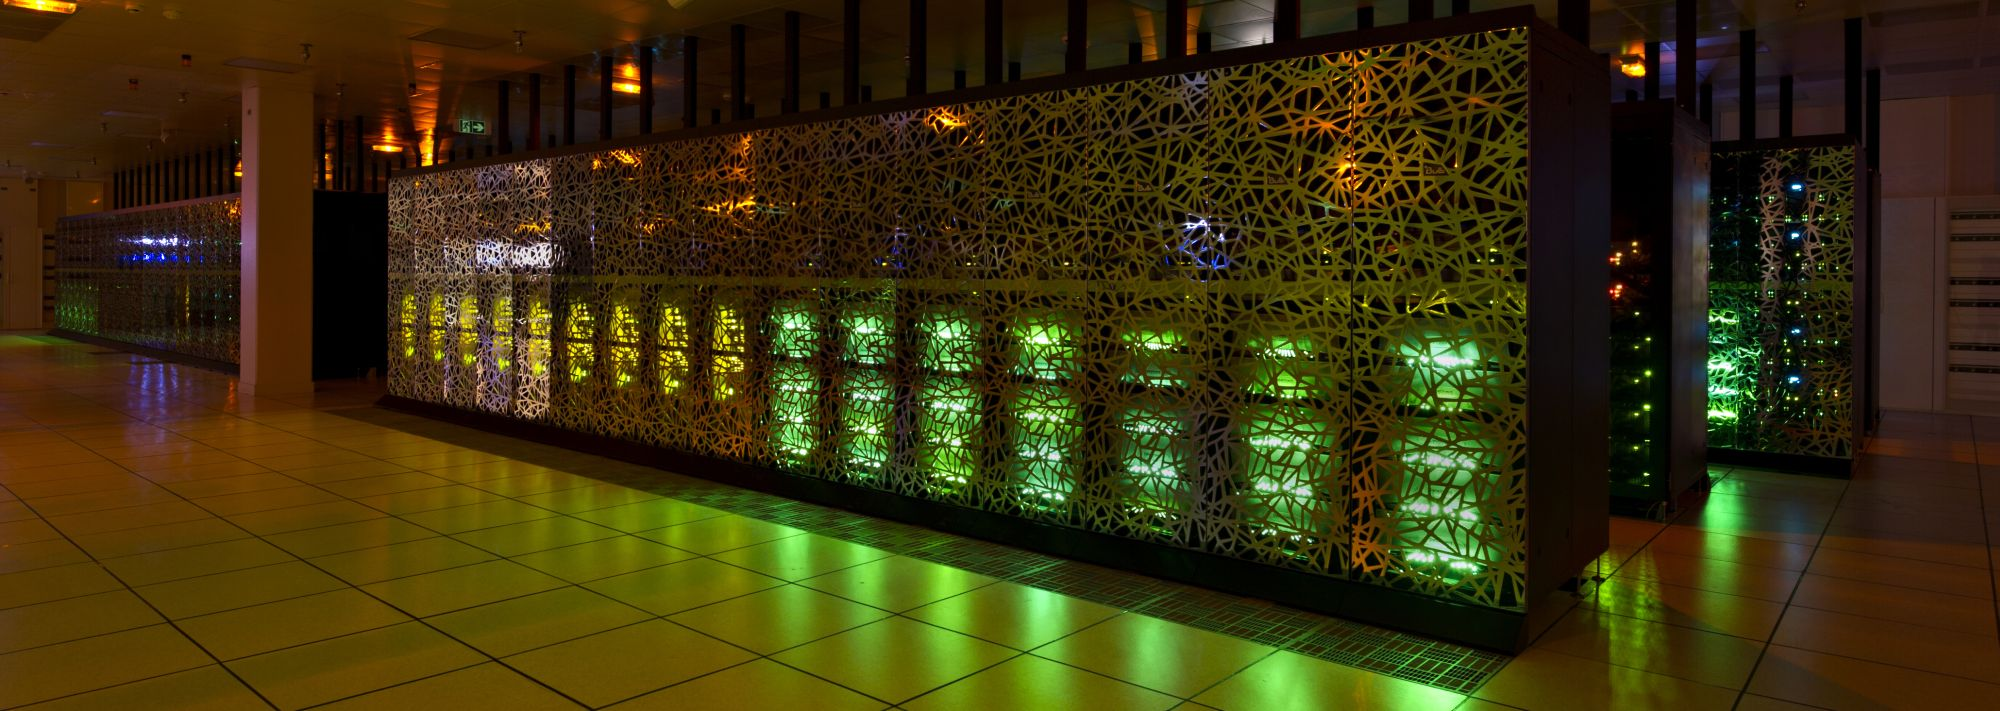
\includegraphics[width=.9\textwidth]{figuras/Supercomputer.jpg}
    \caption{Exemplo de figura embutida no texto}
    \label{fig:supercomputador}
\end{figure}

Aqui um exemplo de como referenciar a Tabela~\ref{tab:tabela_1}. Note que é preciso definir um rótulo (\textit{label}) dentro do comando de definição da tabela.

% Veja a seguir um exemplo de Tabela.
% Você pode usar o site http://www.tablesgenerator.com
% para gerar as tabelas em LaTeX.
\begin{table}[!htp]
\caption[Legenda curta da tabela]{Legenda longa e mais detalhada da tabela.}
\label{tab:tabela_1}
\begin{center}
\begin{tabular}{cc}
\toprule % Linha superior
Coluna 1 & Coluna2 \\ \midrule % Linha do meio 
a & b \\
c & d \\
e & f \\\bottomrule % Linha inferior
\end{tabular}
\end{center}
\end{table}
%
%% Capítulo com os resultados esperados do projeto.
\chapter{Resultados esperados}\label{chp:resultadosEsparados}
O que será criado ou produzido como resultado do projeto proposto?
%
%% Capítulo com os Desafios científicos e tecnológicos e os meios e métodos para superá-los.
\chapter{Desafios científicos e tecnológicos e os meios e métodos para superá-los}\label{chp:desafios}

Explicite os desafios científicos e tecnológicos que o projeto se propõe a superar para atingir os objetivos. Descreva com que meios e métodos estes desafios poderão ser vencidos. Cite referências que ajudem os assessores que analisarão a proposta a entenderem que os desafios mencionados não foram ainda vencidos (ou ainda não foram vencidos de forma adequada) e que poderão ser vencidos com os métodos e meios da proposta em análise.
%
%% Capítulo com o Cronograma.
\chapter{Cronograma}\label{chp:cronograma}

Quando o projeto será completado? Quais os eventos marcantes que poderão ser usados para medir o progresso do projeto e quando estará completo? Caso o projeto proposto seja parte de outro projeto maior já em andamento, estime os prazos somente para o projeto proposto.
%
%% Capítulo com Disseminação e avaliação.
\chapter{Disseminação e avaliação}\label{chp:disseminacao}

Como os resultados do projeto deverão ser avaliados e como serão disseminados?

%
%% Capítulo com Outros apoios.
\chapter{Outros apoios}\label{chp:outrosApoios}
Demonstre outros apoios ao projeto, se houver, em forma de fundos, bens ou serviços, mas sem incluir itens como uso de instalações da instituição que já estão disponíveis. Note que os autores das propostas selecionadas deverão apresentar carta oficial assinada pelo dirigente da instituição, comprometendo os recursos e bens adicionais descritos na proposta.
%
%% Referências bibliográficas
\printbibliography[heading=bibintoc, % Adiciona no sumário
                   title={Referências bibliográficas} % Nome do Capítulo
                  ]
%% Fim do documento
\end{document}
